\begin{center}
  \textsf{Листок 7.}
\end{center}
\vspace{0.01mm}
\nopagebreak[2]

\taskpic{ 
Два одинаковых кубика с длиной ребра $b$ массой $m$ каждый
  стоят на горизонтальном столе, на расстоянии $b$ друг от друга. Между
  ними помещён рычаг длиной $2^{3/2}b$ с пренебрежимо малой
  массой. Коэффициент трения между поверхностями кубиков и столом
  $k$. Коэффициент трения между рычагом и кубиками очень большой в точке
  $A$ и очень маленький в точке $C$. В точке $B$ приложена сила $F$,
  направленная перпендикулярно рычагу как показано на
  рисунке. Определите, какой из кубиков сдвигается раньше, если
  постепенно увеличивать силу $F$.  }
{ 
\begin{tikzpicture}[>=stealth,scale=0.45]
    \draw (-0.4,0) -- (6.4,0);
    \draw[brown,thick] (0,0) rectangle ++(2,2) ++(2,-2) rectangle ++(2,2);
    \coordinate (a) at (2,0);
    \coordinate (f) at ($(a)!5.6!45:(3,0)$);
    \draw[thick] (a) -- (f);
    \draw[->] (f) -- ++(-45:1) node[below] {$\vec{F}$};
  \end{tikzpicture}
%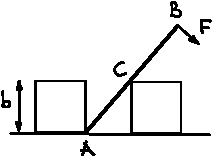
\includegraphics[width=4cm]{p09_26.pdf}
}

\taskpic{ Однородный стрежень длиной $l$ опирается о пол и
  ступеньку. Коэффициент трения между стержнем и полом равен 1, трения
  между стержнем и ступенькой нет. При какой высоте ступеньки стержень
  может находиться в равновесии, если угол $\alpha = \pi /4$?
}{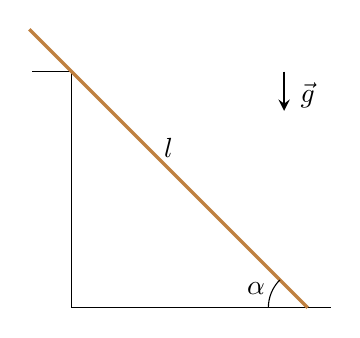
\begin{tikzpicture}[>=stealth,scale=1]
\draw (-0.5,3) -- (0,3) -- (0,0) -- (3.3,0);
\draw[brown, very thick] (3,0) -- +(135:5) node[black,midway, above] {$l$};
\draw[black] (3,0) +(135:0.5) arc (135:180:0.5);
\path (3,0) + (160:0.7) node{$\alpha$};
\draw[thick,->] (2.7,3) -- (2.7,2.5);
\path (3,2.7) node {$\vec{g}$};
\end{tikzpicture}
%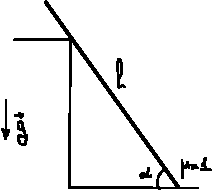
\includegraphics[width=4cm]{p09_27.pdf}
}

\taskpic{ В системе, изображённой на рисунке, трение в блоках и между
  другими поверхностями отсутствует. Если грузу массой $m$ позволить
  двигаться, то за какое время он достигает подставки? Начальная
  скорость груза равна нулю, начальное расстояние от груза до
  подставки $h$, нить невесомая и нерастяжимая. Масса подставки $M$.
}{
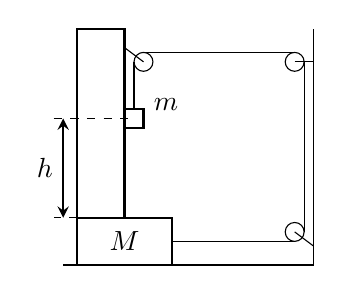
\begin{tikzpicture}[>=stealth,scale=0.6]
  \draw (-0.3,0) -- ++(5.3,0) -- ++ (0,5);
  \draw[thick] (0,0) rectangle (2,1) node[midway] {$M$};
  \draw[thick] (0,1) rectangle (1,5);
  \draw (2,0.5) -- (4.6,0.5);
  \filldraw[white,draw=black] (4.6,0.7) circle (0.2);
  \draw (4.6,0.7) -- ++(0.4,-0.3);
  \draw (4.8,0.7) -- ++(0,3.6);
  \filldraw[white,draw=black] (4.6,4.3) circle (0.2);
  \draw (4.6,4.3) -- ++(0.4,0);
  \draw (4.6,4.5) -- ++(-3.2,0);
  \filldraw[white,draw=black] (1.4,4.3) circle (0.2);
  \draw (1.4,4.3) -- ++(-0.4,0.3);
  \draw (1.2,4.3) -- ++(0,-1);
  \draw[thick] (1,3.3) rectangle ++(0.4,-0.4) node[above=0.3cm,right]
  {$m$};
  \draw[dashed] (0,1) -- ++(-0.5,0) ++ (0,2.1) -- ++(1.7,0);
  \draw[thick,<->] (-0.3,1) -- ++(0,2.1) node[midway,left] {$h$};
\end{tikzpicture}
%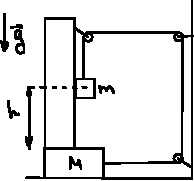
\includegraphics[width=4cm]{p09_28.pdf}
}

\taskpic{ Найдите ускорение грузов, если масса каждого груза равна
  $m$. Массами нитей и блоков пренебречь, нити нерастяжимы, трение
  отсутствует.
}{
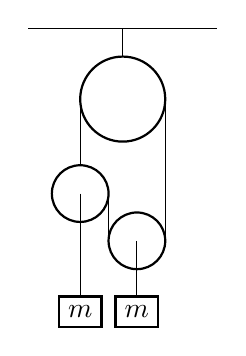
\begin{tikzpicture}[scale=0.6]
  \draw (1,0) -- (5,0) (3,0) -- (3,-1.5);
  \filldraw[thick,white,draw=black] (3,-1.5) circle (0.9);
  \draw (2.1,-1.5) -- ++(0,-2) (3.9,-1.5) -- ++(0,-3);
  \filldraw[thick,white,draw=black] (2.1,-3.5) circle (0.6);
  \filldraw[thick,white,draw=black] (3.3,-4.5) circle (0.6);
  \draw (2.7,-3.5) -- +(0,-1);
  \draw (2.1,-3.5) -- +(0,-2.5);
  \draw (3.3,-4.5) -- +(0,-1.5);
  \node [rectangle,fill=white,draw=black,minimum height=0.7,thick] at
  (2.1,-6) {$m$};
  \node [rectangle,fill=white,draw=black,minimum height=0.7,thick] at
  (3.3,-6) {$m$};
\end{tikzpicture}
%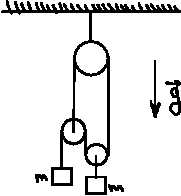
\includegraphics[width=4cm]{p09_29.pdf}
}
